% Options for packages loaded elsewhere
\PassOptionsToPackage{unicode}{hyperref}
\PassOptionsToPackage{hyphens}{url}
\PassOptionsToPackage{dvipsnames,svgnames,x11names}{xcolor}
%
\documentclass[
  letterpaper,
  DIV=11,
  numbers=noendperiod]{scrartcl}

\usepackage{amsmath,amssymb}
\usepackage{lmodern}
\usepackage{iftex}
\ifPDFTeX
  \usepackage[T1]{fontenc}
  \usepackage[utf8]{inputenc}
  \usepackage{textcomp} % provide euro and other symbols
\else % if luatex or xetex
  \usepackage{unicode-math}
  \defaultfontfeatures{Scale=MatchLowercase}
  \defaultfontfeatures[\rmfamily]{Ligatures=TeX,Scale=1}
\fi
% Use upquote if available, for straight quotes in verbatim environments
\IfFileExists{upquote.sty}{\usepackage{upquote}}{}
\IfFileExists{microtype.sty}{% use microtype if available
  \usepackage[]{microtype}
  \UseMicrotypeSet[protrusion]{basicmath} % disable protrusion for tt fonts
}{}
\makeatletter
\@ifundefined{KOMAClassName}{% if non-KOMA class
  \IfFileExists{parskip.sty}{%
    \usepackage{parskip}
  }{% else
    \setlength{\parindent}{0pt}
    \setlength{\parskip}{6pt plus 2pt minus 1pt}}
}{% if KOMA class
  \KOMAoptions{parskip=half}}
\makeatother
\usepackage{xcolor}
\setlength{\emergencystretch}{3em} % prevent overfull lines
\setcounter{secnumdepth}{-\maxdimen} % remove section numbering
% Make \paragraph and \subparagraph free-standing
\ifx\paragraph\undefined\else
  \let\oldparagraph\paragraph
  \renewcommand{\paragraph}[1]{\oldparagraph{#1}\mbox{}}
\fi
\ifx\subparagraph\undefined\else
  \let\oldsubparagraph\subparagraph
  \renewcommand{\subparagraph}[1]{\oldsubparagraph{#1}\mbox{}}
\fi

\usepackage{color}
\usepackage{fancyvrb}
\newcommand{\VerbBar}{|}
\newcommand{\VERB}{\Verb[commandchars=\\\{\}]}
\DefineVerbatimEnvironment{Highlighting}{Verbatim}{commandchars=\\\{\}}
% Add ',fontsize=\small' for more characters per line
\usepackage{framed}
\definecolor{shadecolor}{RGB}{241,243,245}
\newenvironment{Shaded}{\begin{snugshade}}{\end{snugshade}}
\newcommand{\AlertTok}[1]{\textcolor[rgb]{0.68,0.00,0.00}{#1}}
\newcommand{\AnnotationTok}[1]{\textcolor[rgb]{0.37,0.37,0.37}{#1}}
\newcommand{\AttributeTok}[1]{\textcolor[rgb]{0.40,0.45,0.13}{#1}}
\newcommand{\BaseNTok}[1]{\textcolor[rgb]{0.68,0.00,0.00}{#1}}
\newcommand{\BuiltInTok}[1]{\textcolor[rgb]{0.00,0.23,0.31}{#1}}
\newcommand{\CharTok}[1]{\textcolor[rgb]{0.13,0.47,0.30}{#1}}
\newcommand{\CommentTok}[1]{\textcolor[rgb]{0.37,0.37,0.37}{#1}}
\newcommand{\CommentVarTok}[1]{\textcolor[rgb]{0.37,0.37,0.37}{\textit{#1}}}
\newcommand{\ConstantTok}[1]{\textcolor[rgb]{0.56,0.35,0.01}{#1}}
\newcommand{\ControlFlowTok}[1]{\textcolor[rgb]{0.00,0.23,0.31}{#1}}
\newcommand{\DataTypeTok}[1]{\textcolor[rgb]{0.68,0.00,0.00}{#1}}
\newcommand{\DecValTok}[1]{\textcolor[rgb]{0.68,0.00,0.00}{#1}}
\newcommand{\DocumentationTok}[1]{\textcolor[rgb]{0.37,0.37,0.37}{\textit{#1}}}
\newcommand{\ErrorTok}[1]{\textcolor[rgb]{0.68,0.00,0.00}{#1}}
\newcommand{\ExtensionTok}[1]{\textcolor[rgb]{0.00,0.23,0.31}{#1}}
\newcommand{\FloatTok}[1]{\textcolor[rgb]{0.68,0.00,0.00}{#1}}
\newcommand{\FunctionTok}[1]{\textcolor[rgb]{0.28,0.35,0.67}{#1}}
\newcommand{\ImportTok}[1]{\textcolor[rgb]{0.00,0.46,0.62}{#1}}
\newcommand{\InformationTok}[1]{\textcolor[rgb]{0.37,0.37,0.37}{#1}}
\newcommand{\KeywordTok}[1]{\textcolor[rgb]{0.00,0.23,0.31}{#1}}
\newcommand{\NormalTok}[1]{\textcolor[rgb]{0.00,0.23,0.31}{#1}}
\newcommand{\OperatorTok}[1]{\textcolor[rgb]{0.37,0.37,0.37}{#1}}
\newcommand{\OtherTok}[1]{\textcolor[rgb]{0.00,0.23,0.31}{#1}}
\newcommand{\PreprocessorTok}[1]{\textcolor[rgb]{0.68,0.00,0.00}{#1}}
\newcommand{\RegionMarkerTok}[1]{\textcolor[rgb]{0.00,0.23,0.31}{#1}}
\newcommand{\SpecialCharTok}[1]{\textcolor[rgb]{0.37,0.37,0.37}{#1}}
\newcommand{\SpecialStringTok}[1]{\textcolor[rgb]{0.13,0.47,0.30}{#1}}
\newcommand{\StringTok}[1]{\textcolor[rgb]{0.13,0.47,0.30}{#1}}
\newcommand{\VariableTok}[1]{\textcolor[rgb]{0.07,0.07,0.07}{#1}}
\newcommand{\VerbatimStringTok}[1]{\textcolor[rgb]{0.13,0.47,0.30}{#1}}
\newcommand{\WarningTok}[1]{\textcolor[rgb]{0.37,0.37,0.37}{\textit{#1}}}

\providecommand{\tightlist}{%
  \setlength{\itemsep}{0pt}\setlength{\parskip}{0pt}}\usepackage{longtable,booktabs,array}
\usepackage{calc} % for calculating minipage widths
% Correct order of tables after \paragraph or \subparagraph
\usepackage{etoolbox}
\makeatletter
\patchcmd\longtable{\par}{\if@noskipsec\mbox{}\fi\par}{}{}
\makeatother
% Allow footnotes in longtable head/foot
\IfFileExists{footnotehyper.sty}{\usepackage{footnotehyper}}{\usepackage{footnote}}
\makesavenoteenv{longtable}
\usepackage{graphicx}
\makeatletter
\def\maxwidth{\ifdim\Gin@nat@width>\linewidth\linewidth\else\Gin@nat@width\fi}
\def\maxheight{\ifdim\Gin@nat@height>\textheight\textheight\else\Gin@nat@height\fi}
\makeatother
% Scale images if necessary, so that they will not overflow the page
% margins by default, and it is still possible to overwrite the defaults
% using explicit options in \includegraphics[width, height, ...]{}
\setkeys{Gin}{width=\maxwidth,height=\maxheight,keepaspectratio}
% Set default figure placement to htbp
\makeatletter
\def\fps@figure{htbp}
\makeatother

\KOMAoption{captions}{tableheading}
\makeatletter
\makeatother
\makeatletter
\makeatother
\makeatletter
\@ifpackageloaded{caption}{}{\usepackage{caption}}
\AtBeginDocument{%
\ifdefined\contentsname
  \renewcommand*\contentsname{Table of contents}
\else
  \newcommand\contentsname{Table of contents}
\fi
\ifdefined\listfigurename
  \renewcommand*\listfigurename{List of Figures}
\else
  \newcommand\listfigurename{List of Figures}
\fi
\ifdefined\listtablename
  \renewcommand*\listtablename{List of Tables}
\else
  \newcommand\listtablename{List of Tables}
\fi
\ifdefined\figurename
  \renewcommand*\figurename{Figure}
\else
  \newcommand\figurename{Figure}
\fi
\ifdefined\tablename
  \renewcommand*\tablename{Table}
\else
  \newcommand\tablename{Table}
\fi
}
\@ifpackageloaded{float}{}{\usepackage{float}}
\floatstyle{ruled}
\@ifundefined{c@chapter}{\newfloat{codelisting}{h}{lop}}{\newfloat{codelisting}{h}{lop}[chapter]}
\floatname{codelisting}{Listing}
\newcommand*\listoflistings{\listof{codelisting}{List of Listings}}
\makeatother
\makeatletter
\@ifpackageloaded{caption}{}{\usepackage{caption}}
\@ifpackageloaded{subcaption}{}{\usepackage{subcaption}}
\makeatother
\makeatletter
\@ifpackageloaded{tcolorbox}{}{\usepackage[many]{tcolorbox}}
\makeatother
\makeatletter
\@ifundefined{shadecolor}{\definecolor{shadecolor}{rgb}{.97, .97, .97}}
\makeatother
\makeatletter
\makeatother
\ifLuaTeX
  \usepackage{selnolig}  % disable illegal ligatures
\fi
\IfFileExists{bookmark.sty}{\usepackage{bookmark}}{\usepackage{hyperref}}
\IfFileExists{xurl.sty}{\usepackage{xurl}}{} % add URL line breaks if available
\urlstyle{same} % disable monospaced font for URLs
\hypersetup{
  pdftitle={Bias in CLR models: simulation},
  pdfauthor={Koen Van den Berge},
  colorlinks=true,
  linkcolor={blue},
  filecolor={Maroon},
  citecolor={Blue},
  urlcolor={Blue},
  pdfcreator={LaTeX via pandoc}}

\title{Bias in CLR models: simulation}
\author{Koen Van den Berge}
\date{}

\begin{document}
\maketitle
\ifdefined\Shaded\renewenvironment{Shaded}{\begin{tcolorbox}[sharp corners, frame hidden, interior hidden, borderline west={3pt}{0pt}{shadecolor}, boxrule=0pt, enhanced, breakable]}{\end{tcolorbox}}\fi

\hypertarget{set-up}{%
\subsection{Set-up}\label{set-up}}

\begin{enumerate}
\def\labelenumi{\arabic{enumi}.}
\item
  Simulate absolute cell-count abundances using a log-linear model.
\item
  Sample cells from absolute count with probability equal to absolute
  abundance.
\item
  Calculate fold-change on relative counts, and check bias.
\end{enumerate}

\hypertarget{simulation-details}{%
\subsection{Simulation details}\label{simulation-details}}

We simulate the equivalence of a log-linear model with two groups.

\begin{itemize}
\item
  Mean in group1: \(\mu_0 \sim NB(\mu=400, \phi=2)\)
\item
  Log-fold-change on absolute counts
  \(\beta \sim lN(\mu_{\beta}=0), \sigma_{\beta}=2)\)
\item
  Decide which log-fold-changes are different from zero
  \(\beta * B(n=1, \pi_{\beta} = .15) * sign\), where sign is randomly
  selected to be -1 or 1.
\item
  The log-fold-changes represent \(\log(\mu_1/\mu_0) = \beta\). So,
  \(\mu_1 = \exp(\beta) \mu_0\).
\item
  Calculate true relative abundance for each cell type:
  \(\pi_{p0} = \mu_0 / \sum_p \mu_0\), and similarly for condition 1.
\item
  Simulate from a Multinomial
  \(Y_{cip} \sim Mult(n= 1e4, \pi=\pi_{p})\), with \(\pi_p\) being
  either \(\pi_{p0}\) or \(\pi_{p1}\).
\end{itemize}

\begin{Shaded}
\begin{Highlighting}[]
\NormalTok{logit }\OtherTok{\textless{}{-}} \ControlFlowTok{function}\NormalTok{(x) }\FunctionTok{log}\NormalTok{(x}\SpecialCharTok{/}\NormalTok{(}\DecValTok{1}\SpecialCharTok{{-}}\NormalTok{x))}
\FunctionTok{set.seed}\NormalTok{(}\DecValTok{49873528}\NormalTok{)}
\NormalTok{n }\OtherTok{\textless{}{-}} \DecValTok{40} \CommentTok{\# sample size}
\NormalTok{P }\OtherTok{\textless{}{-}} \DecValTok{10} \CommentTok{\# number of cell types}
\NormalTok{mu0 }\OtherTok{\textless{}{-}} \FunctionTok{rnbinom}\NormalTok{(}\AttributeTok{n=}\NormalTok{P, }\AttributeTok{size=}\DecValTok{1}\SpecialCharTok{/}\DecValTok{2}\NormalTok{, }\AttributeTok{mu=}\DecValTok{400}\NormalTok{)}
\NormalTok{mu0 }\CommentTok{\# absolute counts in group 0}
\end{Highlighting}
\end{Shaded}

\begin{verbatim}
 [1]  48 281 430   3 260 413 711 739   0  40
\end{verbatim}

\begin{Shaded}
\begin{Highlighting}[]
\NormalTok{beta }\OtherTok{\textless{}{-}} \FunctionTok{rlnorm}\NormalTok{(}\AttributeTok{n=}\NormalTok{P, }\AttributeTok{meanlog =} \DecValTok{0}\NormalTok{, }\AttributeTok{sdlog=}\DecValTok{2}\NormalTok{) }\SpecialCharTok{*} \CommentTok{\# these are log{-}fold{-}changes}
  \FunctionTok{rbinom}\NormalTok{(}\AttributeTok{n=}\NormalTok{P, }\AttributeTok{size=}\DecValTok{1}\NormalTok{, }\AttributeTok{prob=}\NormalTok{.}\DecValTok{15}\NormalTok{) }\SpecialCharTok{*}
  \FunctionTok{sample}\NormalTok{(}\FunctionTok{c}\NormalTok{(}\SpecialCharTok{{-}}\DecValTok{1}\NormalTok{,}\DecValTok{1}\NormalTok{), }\AttributeTok{size=}\NormalTok{P, }\AttributeTok{replace=}\ConstantTok{TRUE}\NormalTok{) }\CommentTok{\# fold change on log scale}
\NormalTok{mu1 }\OtherTok{\textless{}{-}} \FunctionTok{exp}\NormalTok{(beta) }\SpecialCharTok{*}\NormalTok{ mu0 }\CommentTok{\# because we want log(mu2/mu1) = beta}
\FunctionTok{log}\NormalTok{(mu1}\SpecialCharTok{/}\NormalTok{(mu0)) }\CommentTok{\# fold{-}changes OK}
\end{Highlighting}
\end{Shaded}

\begin{verbatim}
 [1]  0.0000000  0.0000000  0.0000000 -2.5287859  0.0000000  0.0000000
 [7]  0.0000000 -0.3171493        NaN  0.0000000
\end{verbatim}

\begin{Shaded}
\begin{Highlighting}[]
\NormalTok{df }\OtherTok{\textless{}{-}} \FunctionTok{data.frame}\NormalTok{(}\AttributeTok{mu=}\FunctionTok{c}\NormalTok{(mu0,mu1),}
                 \AttributeTok{celltype=}\FunctionTok{factor}\NormalTok{(}\FunctionTok{rep}\NormalTok{(}\DecValTok{1}\SpecialCharTok{:}\NormalTok{P,}\DecValTok{2}\NormalTok{)),}
                 \AttributeTok{group=}\FunctionTok{factor}\NormalTok{(}\FunctionTok{rep}\NormalTok{(}\DecValTok{0}\SpecialCharTok{:}\DecValTok{1}\NormalTok{,}\AttributeTok{each=}\NormalTok{P)))}
\FunctionTok{ggplot}\NormalTok{(df, }\FunctionTok{aes}\NormalTok{(}\AttributeTok{x=}\NormalTok{group, }\AttributeTok{y=}\FunctionTok{log1p}\NormalTok{(mu), }\AttributeTok{group=}\NormalTok{celltype, }\AttributeTok{col=}\NormalTok{celltype)) }\SpecialCharTok{+}
  \FunctionTok{geom\_line}\NormalTok{()}
\end{Highlighting}
\end{Shaded}

\begin{figure}[H]

{\centering 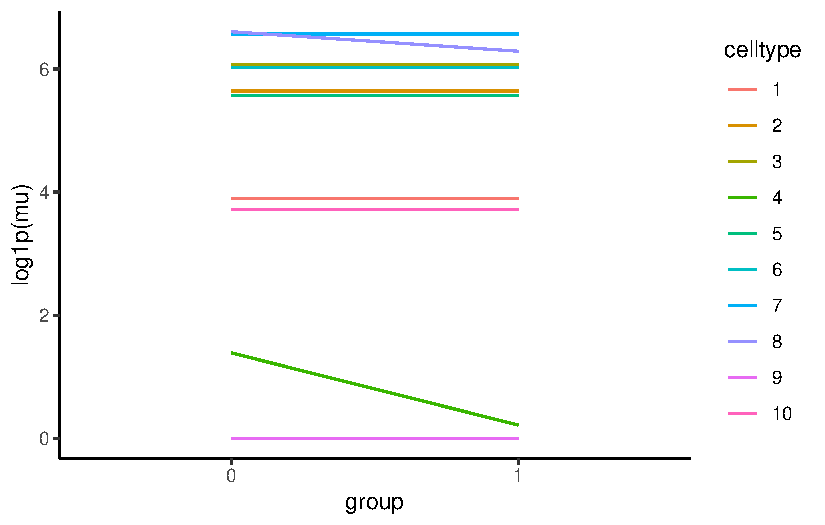
\includegraphics{221215_simulationCLRBias_files/figure-pdf/unnamed-chunk-2-1.pdf}

}

\end{figure}

\begin{Shaded}
\begin{Highlighting}[]
\DocumentationTok{\#\# relative abundances}
\NormalTok{relAbundances }\OtherTok{\textless{}{-}} \FunctionTok{data.frame}\NormalTok{(}\AttributeTok{g0=}\NormalTok{mu0}\SpecialCharTok{/}\FunctionTok{sum}\NormalTok{(mu0),}
                            \AttributeTok{g1=}\NormalTok{mu1}\SpecialCharTok{/}\FunctionTok{sum}\NormalTok{(mu1)) }\CommentTok{\# relative abundance of absolute count}
\FunctionTok{plot}\NormalTok{(}\FunctionTok{logit}\NormalTok{(relAbundances),}\AttributeTok{col=}\FunctionTok{as.numeric}\NormalTok{(beta}\SpecialCharTok{==}\DecValTok{0}\NormalTok{)}\SpecialCharTok{+}\DecValTok{1}\NormalTok{)}
\end{Highlighting}
\end{Shaded}

\begin{figure}[H]

{\centering 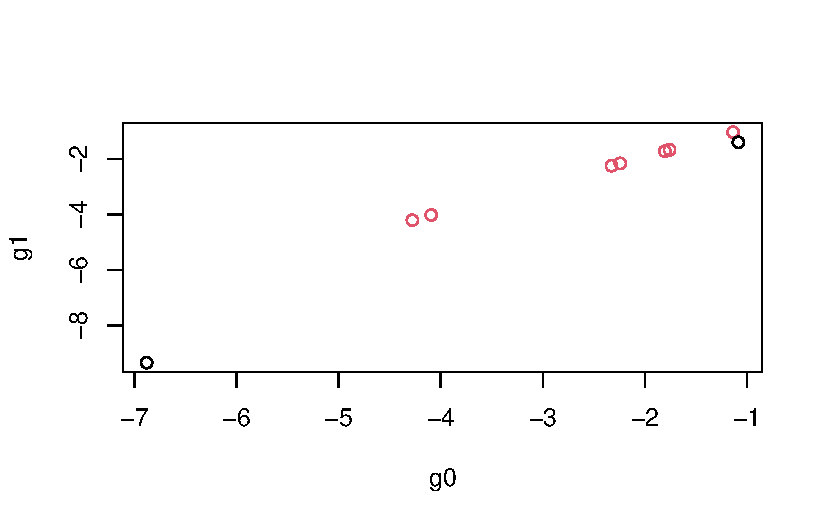
\includegraphics{221215_simulationCLRBias_files/figure-pdf/unnamed-chunk-2-2.pdf}

}

\end{figure}

\begin{Shaded}
\begin{Highlighting}[]
\CommentTok{\# relative abundance information (observed data in typical experiment)}
\NormalTok{Y0 }\OtherTok{\textless{}{-}} \FunctionTok{rmultinom}\NormalTok{(}\AttributeTok{n=}\DecValTok{10}\NormalTok{, }\AttributeTok{size=}\FloatTok{1e4}\NormalTok{, }\AttributeTok{prob=}\NormalTok{relAbundances}\SpecialCharTok{$}\NormalTok{g0)}
\NormalTok{Y1 }\OtherTok{\textless{}{-}} \FunctionTok{rmultinom}\NormalTok{(}\AttributeTok{n=}\DecValTok{10}\NormalTok{, }\AttributeTok{size=}\FloatTok{1e4}\NormalTok{, }\AttributeTok{prob=}\NormalTok{relAbundances}\SpecialCharTok{$}\NormalTok{g1)}
\end{Highlighting}
\end{Shaded}

\hypertarget{data-analysis}{%
\subsection{Data analysis}\label{data-analysis}}

\hypertarget{voomclr-workflow-no-bias-correction.}{%
\subsubsection{voomCLR workflow: no bias
correction.}\label{voomclr-workflow-no-bias-correction.}}

\begin{Shaded}
\begin{Highlighting}[]
\FunctionTok{source}\NormalTok{(}\StringTok{"\textasciitilde{}/Janssen/methodDevelopment/cellComposition/code/voomCLR/voomCLRWorkflow.R"}\NormalTok{)}
\NormalTok{Y }\OtherTok{\textless{}{-}} \FunctionTok{cbind}\NormalTok{(Y0, Y1)}
\NormalTok{group }\OtherTok{\textless{}{-}} \FunctionTok{factor}\NormalTok{(}\FunctionTok{rep}\NormalTok{(}\DecValTok{0}\SpecialCharTok{:}\DecValTok{1}\NormalTok{, }\AttributeTok{each=}\DecValTok{10}\NormalTok{))}
\NormalTok{design }\OtherTok{\textless{}{-}} \FunctionTok{model.matrix}\NormalTok{(}\SpecialCharTok{\textasciitilde{}}\NormalTok{group)}

\FunctionTok{library}\NormalTok{(limma)}
\NormalTok{v }\OtherTok{\textless{}{-}} \FunctionTok{voomCLR}\NormalTok{(}\AttributeTok{counts =}\NormalTok{ Y,}
             \AttributeTok{design =}\NormalTok{ design,}
             \AttributeTok{lib.size =} \DecValTok{1}\NormalTok{)}
\NormalTok{fit }\OtherTok{\textless{}{-}} \FunctionTok{lmFit}\NormalTok{(v, design)}
\CommentTok{\# fit \textless{}{-} applyBiasCorrection(fit)}
\NormalTok{fit }\OtherTok{\textless{}{-}} \FunctionTok{eBayes}\NormalTok{(fit)}
\FunctionTok{plot}\NormalTok{(}\AttributeTok{x=}\NormalTok{fit}\SpecialCharTok{$}\NormalTok{coefficients[,}\DecValTok{2}\NormalTok{], }\AttributeTok{y=}\NormalTok{beta,}
     \AttributeTok{xlab=}\StringTok{"Estimated log{-}fold{-}change"}\NormalTok{,}
     \AttributeTok{ylab=}\StringTok{"True log{-}fold{-}change"}\NormalTok{) ; }\FunctionTok{abline}\NormalTok{(}\DecValTok{0}\NormalTok{,}\DecValTok{1}\NormalTok{,}\AttributeTok{col=}\StringTok{"red"}\NormalTok{)}
\end{Highlighting}
\end{Shaded}

\begin{figure}[H]

{\centering 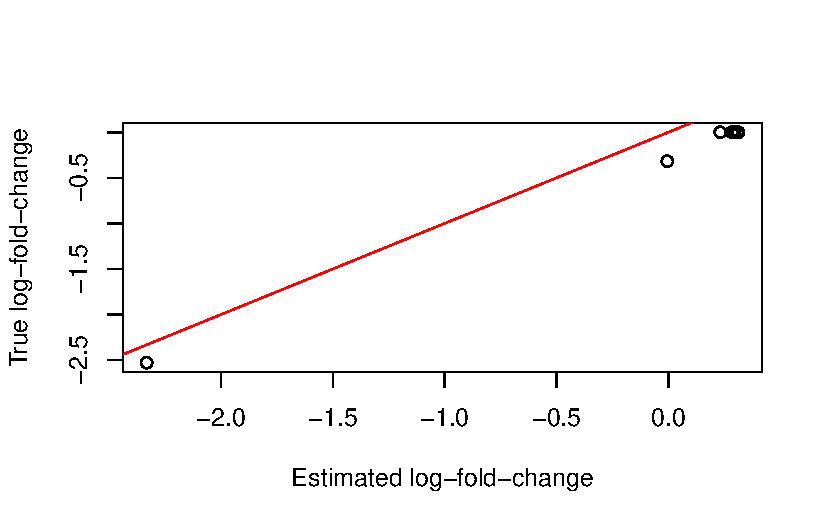
\includegraphics{221215_simulationCLRBias_files/figure-pdf/unnamed-chunk-3-1.pdf}

}

\end{figure}

\begin{Shaded}
\begin{Highlighting}[]
\FunctionTok{boxplot}\NormalTok{(fit}\SpecialCharTok{$}\NormalTok{coefficients[,}\DecValTok{2}\NormalTok{] }\SpecialCharTok{{-}}\NormalTok{ beta, }\AttributeTok{ylim=}\FunctionTok{c}\NormalTok{(}\SpecialCharTok{{-}}\FloatTok{0.4}\NormalTok{,}\FloatTok{0.4}\NormalTok{),}
        \AttributeTok{ylab=}\StringTok{"Difference (estimated{-}true LFC)"}\NormalTok{); }\FunctionTok{abline}\NormalTok{(}\AttributeTok{h=}\DecValTok{0}\NormalTok{, }\AttributeTok{col=}\StringTok{"red"}\NormalTok{, }\AttributeTok{lty=}\DecValTok{2}\NormalTok{)}
\end{Highlighting}
\end{Shaded}

\begin{figure}[H]

{\centering 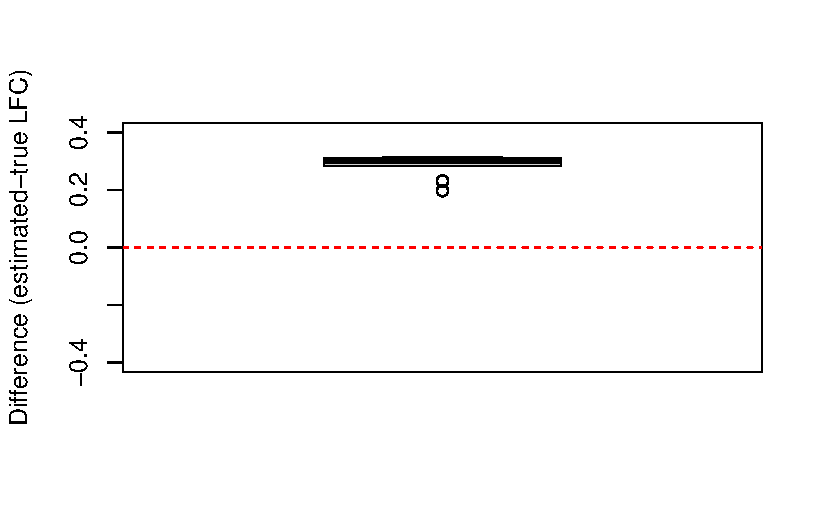
\includegraphics{221215_simulationCLRBias_files/figure-pdf/unnamed-chunk-3-2.pdf}

}

\end{figure}

\hypertarget{bias-correction}{%
\subsubsection{Bias correction}\label{bias-correction}}

\begin{Shaded}
\begin{Highlighting}[]
\FunctionTok{library}\NormalTok{(limma)}
\NormalTok{v }\OtherTok{\textless{}{-}} \FunctionTok{voomCLR}\NormalTok{(}\AttributeTok{counts =}\NormalTok{ Y,}
             \AttributeTok{design =}\NormalTok{ design,}
             \AttributeTok{lib.size =} \DecValTok{1}\NormalTok{)}
\NormalTok{fit }\OtherTok{\textless{}{-}} \FunctionTok{lmFit}\NormalTok{(v, design)}
\NormalTok{fit }\OtherTok{\textless{}{-}} \FunctionTok{applyBiasCorrection}\NormalTok{(fit)}
\NormalTok{fit }\OtherTok{\textless{}{-}} \FunctionTok{eBayes}\NormalTok{(fit)}
\FunctionTok{plot}\NormalTok{(}\AttributeTok{x=}\NormalTok{fit}\SpecialCharTok{$}\NormalTok{coefficients[,}\DecValTok{2}\NormalTok{], }\AttributeTok{y=}\NormalTok{beta,}
     \AttributeTok{xlab=}\StringTok{"Estimated log{-}fold{-}change"}\NormalTok{,}
     \AttributeTok{ylab=}\StringTok{"True log{-}fold{-}change"}\NormalTok{) ; }\FunctionTok{abline}\NormalTok{(}\DecValTok{0}\NormalTok{,}\DecValTok{1}\NormalTok{,}\AttributeTok{col=}\StringTok{"red"}\NormalTok{)}
\end{Highlighting}
\end{Shaded}

\begin{figure}[H]

{\centering 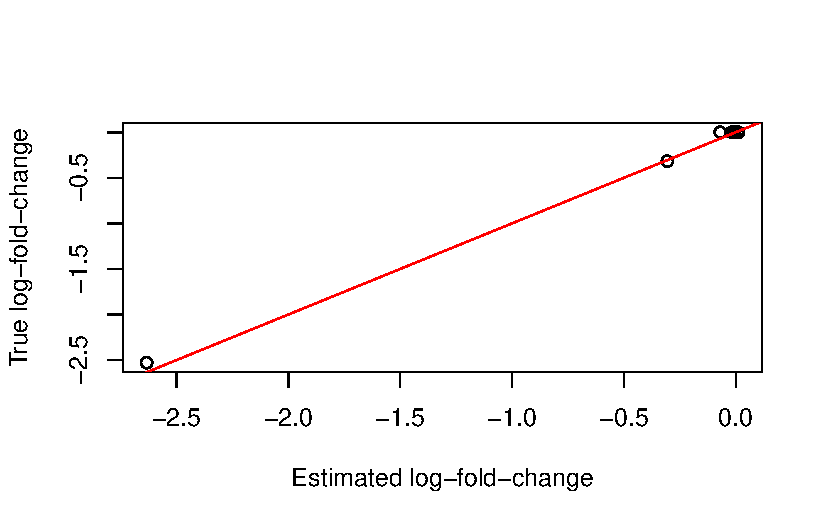
\includegraphics{221215_simulationCLRBias_files/figure-pdf/unnamed-chunk-4-1.pdf}

}

\end{figure}

\begin{Shaded}
\begin{Highlighting}[]
\FunctionTok{boxplot}\NormalTok{(fit}\SpecialCharTok{$}\NormalTok{coefficients[,}\DecValTok{2}\NormalTok{] }\SpecialCharTok{{-}}\NormalTok{ beta, }\AttributeTok{ylim=}\FunctionTok{c}\NormalTok{(}\SpecialCharTok{{-}}\FloatTok{0.4}\NormalTok{,}\FloatTok{0.4}\NormalTok{),}
        \AttributeTok{ylab=}\StringTok{"Difference (estimated{-}true LFC)"}\NormalTok{); }\FunctionTok{abline}\NormalTok{(}\AttributeTok{h=}\DecValTok{0}\NormalTok{, }\AttributeTok{col=}\StringTok{"red"}\NormalTok{, }\AttributeTok{lty=}\DecValTok{2}\NormalTok{)}
\end{Highlighting}
\end{Shaded}

\begin{figure}[H]

{\centering 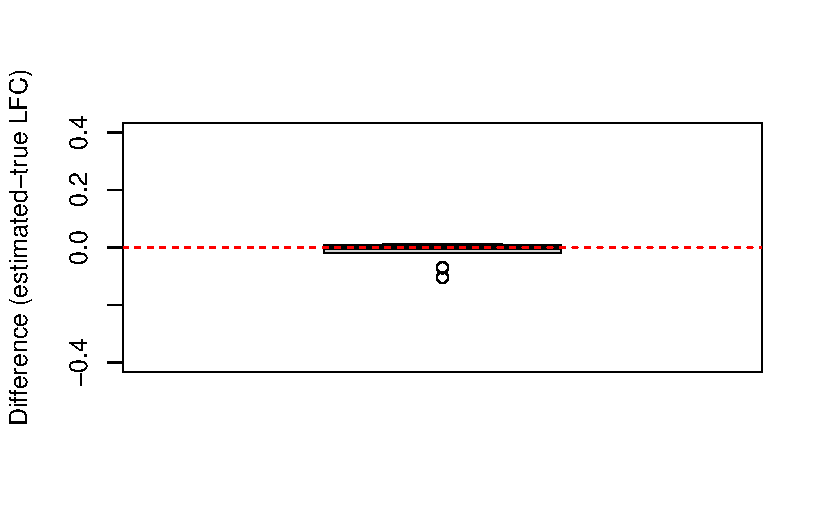
\includegraphics{221215_simulationCLRBias_files/figure-pdf/unnamed-chunk-4-2.pdf}

}

\end{figure}



\end{document}
